\begin{enumerate}[label=]
    \item 
        to find the roots of $f(x) = x^4 - x^2 - 1$ first we find the roots of $g(y) = y^2 - y - 1$.
        which is $\frac{1 \pm\sqrt{5}}{2}$. therefore the roots of $f(x)$ are $\pm \sqrt{\frac{1 \pm \sqrt{5}}{2}}$
        suppose $K$ is the splitting field of $f$ over $\mathbb Q$.
        this means that $\sqrt{\frac{1 + \sqrt{5}}{2}}, \sqrt{\frac{1 - \sqrt{5}}{2}} \in K$.
        which means $\sqrt{\frac{1 + \sqrt{5}}{2}} \sqrt{\frac{1 - \sqrt{5}}{2}} = \sqrt{\frac{1 - 5}{4}} = i \in K$.
        this shows that $\mathbb Q(i, \sqrt{\frac{1 + \sqrt{5}}{2}})$ includes all the roots of $f$ and is also the smallest field therefore it is the splittnig field of $f$.
        and since $[\mathbb Q(\sqrt{\frac{1 + \sqrt{5}}{2}}): \mathbb Q] = 4$ and $i \notin \mathbb Q(\sqrt{\frac{1 + \sqrt{5}}{2}})$ therefore $[K:\mathbb Q] = 8$.
        and since $K$ is seperable over $\mathbb Q$ then $K / \mathbb Q$ is galois and this means that group of automorphisms has 8 elements.
        and since for $i$ we have two possible maps and for $\sqrt{\frac{1 + \sqrt{5}}{2}}$ has four possible maps therefore all of them are automorphisms.
        now let:
        \begin{gather*}
            \delta :
            \begin{cases}
                i \mapsto -i \\
                \sqrt{\frac{1 + \sqrt{5}}{2}} \mapsto  \sqrt{\frac{1 + \sqrt{5}}{2}}
            \end{cases} \
            \tau :
            \begin{cases}
                i \mapsto -i \\
                \sqrt{\frac{1 + \sqrt{5}}{2}} \mapsto -\sqrt{\frac{1 - \sqrt{5}}{2}}
            \end{cases} 
        \end{gather*}
        it is easy to see that $\delta^2 = \tau^4 = 1$. also:
        \begin{gather*}
            \tau \delta:
            \begin{cases}
                i \mapsto i \\
                \sqrt{\frac{1 + \sqrt{5}}{2}} \mapsto  -\sqrt{\frac{1 - \sqrt{5}}{2}}
            \end{cases} \
            \delta \tau^3: 
            \begin{cases}
                i \mapsto i \\
                \sqrt{\frac{1 + \sqrt{5}}{2}} \mapsto  -\sqrt{\frac{1 - \sqrt{5}}{2}}
            \end{cases}
        \end{gather*}
        this shows that $\tau \delta = \delta \tau^{-1}$ which means this group is $D_{2n}$ for $n = 4$.
        this means that all of the elements are:
        \begin{center}
            $
            id:
            \begin{cases}
                i \mapsto i \\
                \sqrt{\frac{1 + \sqrt{5}}{2}} \mapsto  \sqrt{\frac{1 + \sqrt{5}}{2}}
            \end{cases} \
            \delta:
            \begin{cases}
                i \mapsto -i \\
                \sqrt{\frac{1 + \sqrt{5}}{2}} \mapsto  \sqrt{\frac{1 + \sqrt{5}}{2}}
            \end{cases}$ \\
            $\tau:
            \begin{cases}
                i \mapsto -i \\
                \sqrt{\frac{1 + \sqrt{5}}{2}} \mapsto  -\sqrt{\frac{1 - \sqrt{5}}{2}}
            \end{cases} \ 
            \tau \delta:
            \begin{cases}
                i \mapsto i \\ 
                \sqrt{\frac{1 + \sqrt{5}}{2}} \mapsto  -\sqrt{\frac{1 - \sqrt{5}}{2}}
            \end{cases}$ \\
            $\tau^2:
            \begin{cases}
                i \mapsto i \\
                \sqrt{\frac{1 + \sqrt{5}}{2}} \mapsto  -\sqrt{\frac{1 + \sqrt{5}}{2}}
            \end{cases} \ 
            \tau^2 \delta:
            \begin{cases}
                i \mapsto -i \\
                \sqrt{\frac{1 + \sqrt{5}}{2}} \mapsto  -\sqrt{\frac{1 + \sqrt{5}}{2}}
            \end{cases}$ \\
            $ \tau^3:
            \begin{cases}
                i \mapsto -i \\
                \sqrt{\frac{1 + \sqrt{5}}{2}} \mapsto  \sqrt{\frac{1 - \sqrt{5}}{2}}
            \end{cases} \ 
            \tau^3 \delta:
            \begin{cases}
                i \mapsto i \\
                \sqrt{\frac{1 + \sqrt{5}}{2}} \mapsto  \sqrt{\frac{1 - \sqrt{5}}{2}}
            \end{cases}$
        \end{center}
        and the lattice of the group would be:
        \begin{center}
            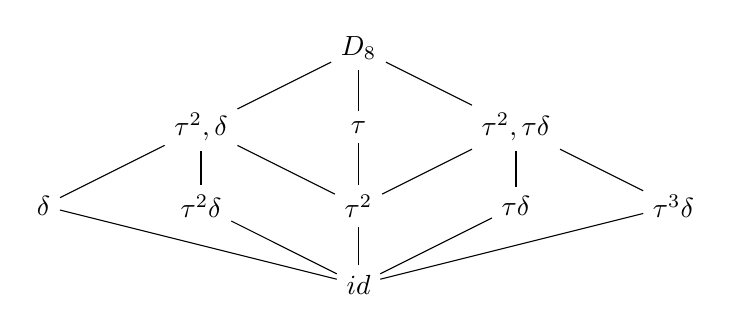
\begin{tikzpicture}
                %nodes 
                \node at (0, 0) (A1) {$id$};
                \node at (0, 1) (A2) {$\braket{\tau^2}$};
                \node at (0, 2) (A3) {$\braket{\tau}$};
                \node at (0, 3) (A4) {$D_8$};
                \node at (-2, 1) (A5) {$\braket{\tau^2 \delta}$};
                \node at (2, 1) (A6) {$\braket{\tau \delta}$};
                \node at (-4, 1) (A7) {$\braket{\delta}$};
                \node at (4, 1) (A8) {$\braket{\tau^3 \delta}$};
                \node at (-2, 2) (A9) {$\braket{\tau^2, \delta}$};
                \node at (2, 2) (A10) {$\braket{\tau^2, \tau \delta}$};
                
                %lines
                \draw (A1)--(A2);
                \draw (A1)--(A5);
                \draw (A1)--(A6);
                \draw (A1)--(A7);
                \draw (A1)--(A8);
                \draw (A2)--(A3);
                \draw (A2)--(A9);
                \draw (A2)--(A10);
                \draw (A5)--(A9);
                \draw (A7)--(A9);
                \draw (A6)--(A10);
                \draw (A8)--(A10);
                \draw (A3)--(A4);
                \draw (A9)--(A4);
                \draw (A10)--(A4);
            \end{tikzpicture}
        \end{center}
        now if we let $\alpha = \sqrt{\frac{1 + \sqrt{5}}{2}}$ and $\beta = \sqrt{\frac{1 - \sqrt{5}}{2}}$ we would have:
        $\tau(\alpha) = -\beta$, $\tau(-\beta) = -\alpha$, $\tau(-\alpha) = \beta$ and $\tau(\beta) = \alpha$. also $\alpha \beta = i$.
        and it is obvious that $\{1, \alpha, \alpha^2, \alpha^3\}$ are a basis for $\mathbb Q(\alpha)$ over $\mathbb Q$ and therefore 
        $\{1, i, \alpha, \alpha i, \alpha^2, \alpha^2 i, \alpha^3, \alpha^3 i\}$ is a basis for $\mathbb Q(\alpha, i)$ over $\mathbb Q$.
        now with this information it is easy to check the coefficient of each eleemnt in form of basis to check whether they are in the fixed field of a subgroup or not:
        \begin{center}
            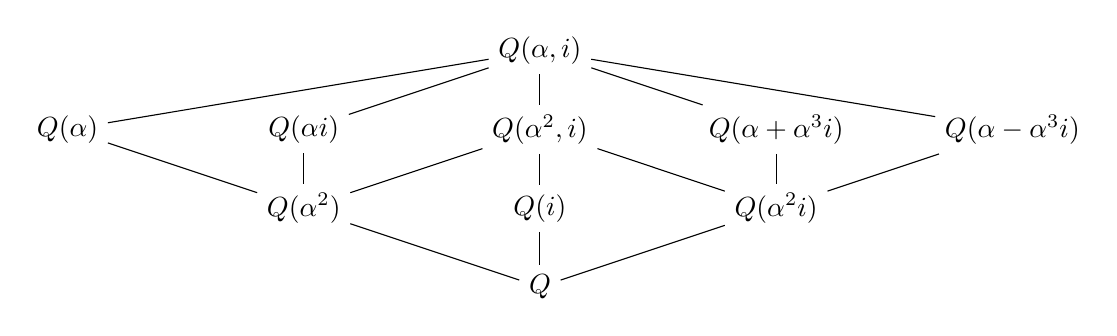
\begin{tikzpicture}
                %nodes
                \node at (0, 3) (A1) {$\mathbb Q(\alpha, i)$};
                \node at (0, 2) (A2) {$\mathbb Q(\alpha^2, i)$};
                \node at (0, 1) (A3) {$\mathbb Q(i)$};
                \node at (0, 0) (A4) {$\mathbb Q$};
                \node at (-3, 2) (A5) {$\mathbb Q(\alpha i)$};
                \node at (3, 2) (A6) {$\mathbb Q(\alpha + \alpha^3 i)$};
                \node at (-6, 2) (A7) {$\mathbb Q(\alpha)$};
                \node at (6, 2) (A8) {$\mathbb Q(\alpha - \alpha^3 i)$};
                \node at (-3, 1) (A9) {$\mathbb Q(\alpha^2)$};
                \node at (3, 1) (A10) {$\mathbb Q(\alpha^2 i)$};
                
                %lines
                \draw (A1)--(A2);
                \draw (A1)--(A5);
                \draw (A1)--(A6);
                \draw (A1)--(A7);
                \draw (A1)--(A8);
                \draw (A2)--(A3);
                \draw (A2)--(A9);
                \draw (A2)--(A10);
                \draw (A5)--(A9);
                \draw (A7)--(A9);
                \draw (A6)--(A10);
                \draw (A8)--(A10);
                \draw (A3)--(A4);
                \draw (A9)--(A4);
                \draw (A10)--(A4);
            \end{tikzpicture}
        \end{center}
\end{enumerate}